% ECON 5030 midterm study guide: a 4-hour plan built from the 10/22 review notes (midterm.md),
% the Ch1-3 and Ch5 course notes, Problem Sets 1-3, and last year's midterm.
\documentclass[11pt]{article}
\usepackage[letterpaper,margin=1in]{geometry}
\usepackage{amsmath,amssymb}
\usepackage[T1]{fontenc}
\usepackage{lmodern}
\usepackage{cmap}
\usepackage{enumitem}
\usepackage{array,booktabs}
\usepackage[most]{tcolorbox}
\usepackage{tikz}
\usetikzlibrary{trees}
\usepackage[hidelinks]{hyperref}

\setlength{\parindent}{0pt}
\setlength{\parskip}{5pt}
\setlist{itemsep=2pt,topsep=3pt}

\newtcolorbox{defbox}[1]{colback=blue!4,colframe=blue!45!black,fonttitle=\bfseries,title={#1},breakable}
\newtcolorbox{tipbox}{colback=orange!7,colframe=orange!70!black,fonttitle=\bfseries,title={Exam tip},breakable}
\newtcolorbox{workbox}[1]{colback=green!4,colframe=green!40!black,fonttitle=\bfseries,title={#1},breakable}
\newtcolorbox{examq}[1]{colback=purple!3,colframe=purple!55!black,fonttitle=\bfseries,
  title={Expected exam question: #1},breakable,segmentation style={dashed,purple!55!black}}
\newcommand{\soln}{\tcblower\textbf{Solution.}\ }
\newtcolorbox{timebox}[1]{colback=gray!8,colframe=gray!60!black,fonttitle=\bfseries,title={#1},breakable}

\tikzset{dec/.style={circle,fill,inner sep=1.5pt}}

\title{ECON 5030 Midterm Study Guide\\[3pt]\large A 4-hour plan, including Cournot from scratch,\\ with expected exam questions and solutions}
\author{Built from the 10/22 review, the course notes (Ch.\ 1--3, Ch.\ 5), PS1--PS3, and last year's midterm}
\date{}

\begin{document}
\maketitle
\tableofcontents
\newpage

%=====================================================================
\section{What is on the exam, and the 4-hour plan}

\subsection*{What the professor said (10/22 review)}
\begin{itemize}
\item \textbf{Preferences:} define complete and transitive, and know the rationality axioms and when a utility function exists. ``Easier than PS1, more definitions than proofs.''
\item \textbf{Expected utility:} what EU is and what extra assumption it needs (\emph{independence}).
\item \textbf{Normal form:} ``will 100\% ask.'' Know the three parts (players, strategies, payoffs), and how to build one for simultaneous and sequential games.
\item \textbf{Solution concepts:} dominant strategies, rationalizability / iterated deletion, Nash equilibrium (know the definition), and mixed NE.
\item \textbf{Efficiency and equity:} NE is generally neither.
\item \textbf{Market games:} CS, PS, TS, DWL; what blocks pure exchange; what production adds.
\item \textbf{Cournot oligopoly:} ``the biggest of the problems on the exam,'' ``a Cournot example from the problem set will probably be on the exam.''
\item \textbf{Not on the midterm:} neoclassical demand (UMAX/Lagrangian) and Bertrand.
\end{itemize}

\textbf{Last year's midterm} (transcribed in \texttt{ECON5030\_Midterm.pdf}) had four sections: (1) Preferences, (2) Game Theory (a sequential game written out in normal form, plus a money game with ``Case 1/2/3'' preferences), (3) Conceptual, and (4) General equilibrium. Expect the same shape, with Section 4 replaced by Cournot.

\subsection*{The 4-hour schedule}
\begin{center}
\renewcommand{\arraystretch}{1.25}
\begin{tabular}{@{}p{2.1cm}p{9.4cm}p{3.2cm}@{}}
\toprule
\textbf{Time} & \textbf{Do this} & \textbf{Guide section}\\\midrule
0:00--0:25 & Preferences and utility: memorize the definitions, then do the three ``is it complete / transitive / representable?'' drills. & \S2\\
0:25--0:45 & Expected utility and the independence axiom. Write out the answer to ``why exactly independence?'' from memory once. & \S3\\
0:45--1:45 & Game theory: normal form, sequential strategies, IDSDS, NE, SPE, mixed NE. Work every example with pencil, especially the 2-step sequential game recipe. & \S4\\
1:45--1:55 & \textbf{Break.} & \\
1:55--3:10 & \textbf{Cournot from scratch.} Read the recipe, then solve PS3 \#1 and \#2 yourself before looking at the solutions. Draw the BR graph and the welfare graph. & \S5, \S6\\
3:10--3:25 & Market games and welfare: CS/PS/TS/DWL, equity, pure exchange vs.\ production. & \S7\\
3:25--4:00 & \textbf{Timed practice:} Sample Midterm 2, Sections 2.2 and 4 (25 min), then grade with its key (10 min). Finish with the final checklist (\S9). & \S8, \S9\\
\bottomrule
\end{tabular}
\end{center}

\begin{tipbox}
Grading is ``long, just show what you've learnt.'' On every question: \textbf{state the definition first}, then apply it. Definitions are free points, and the professor explicitly rewards them.

Each topic ends with purple \textbf{Expected exam question} boxes in last year's style. Cover the solution (below the dashed line), answer on paper, then check. Budget about a third of each time block for them.
\end{tipbox}

%=====================================================================
\section{Preferences and utility (25 min)}

\begin{defbox}{Core definitions (memorize word for word)}
\begin{itemize}
\item \textbf{Complete:} $(\succsim,S)$ is complete if for all $x,y\in S$, either $x\succsim y$ or $y\succsim x$ (or both).
\item \textbf{Transitive:} $(\succsim,S)$ is transitive if for all $x,y,z\in S$, $x\succsim y$ and $y\succsim z$ imply $x\succsim z$.
\item \textbf{Rational} $=$ complete $+$ transitive.
\item \textbf{Strict preference / indifference:} $x\succ y$ iff $x\succsim y$ and not $y\succsim x$; $x\sim y$ iff $x\succsim y$ and $y\succsim x$.
\item \textbf{Representation:} $u:S\to\mathbb{R}$ represents $(\succsim,S)$ if for all $x,y$: $x\succsim y\iff u(x)\ge u(y)$.
\item \textbf{Continuous:} for any sequences with $x^n\succsim y^n$, $x^n\to x$, $y^n\to y$, we have $x\succsim y$. (No ``jumps'' at limits.)
\end{itemize}
\end{defbox}

\textbf{The existence results (the story the professor wants):}
\begin{enumerate}
\item If $S$ is \textbf{finite} and $\succsim$ is complete and transitive, then an optimal choice exists and a utility function exists. (Rank the indifference classes $1,2,\dots,K$ from worst to best and set $u(x)=$ the rank of $x$'s class.)
\item If $X\subseteq\mathbb{R}^L$ is \textbf{infinite}, complete $+$ transitive is \emph{not} enough. You also need \textbf{continuity}. Complete $+$ transitive $+$ continuous $\Rightarrow$ a continuous utility function exists.
\item Optimal choices $=\arg\max u$.
\item Utility is \textbf{ordinal}: any strictly increasing transformation of $u$ represents the same preferences.
\end{enumerate}

\textbf{The standard counterexample, lexicographic preferences} on $[0,1]^2$: $x\succ y$ if $x_1>y_1$, or $x_1=y_1$ and $x_2>y_2$. These are complete and transitive but \emph{not continuous}: $(1/n,0)\succ(0,1)$ for every $n$, but the limit $(0,0)\prec(0,1)$. No utility function exists. (Intuition: each $x_1$ needs its own disjoint utility interval, and there are uncountably many of them but only countably many rationals to tag them with.)

\textbf{Two facts that answer ``does a utility function exist?'' instantly:}
\begin{itemize}
\item A represented preference is always \emph{complete} (real numbers are always comparable).
\item A represented preference is always \emph{transitive} ($\ge$ on reals is transitive).
\end{itemize}
So if either property fails, the answer is ``no, because\ldots''

\subsection*{How to check a weird preference (last year's 1.1--1.3)}
\begin{enumerate}
\item \textbf{Completeness:} look for a pair that \emph{no} rule ranks. One counterexample kills it. Try bundles where one coordinate is bigger and the other is smaller, e.g. $(1,0)$ vs.\ $(0,1)$.
\item \textbf{Transitivity:} look for a cycle, or for ``small steps that add up'' (threshold rules).
\item \textbf{Utility:} fails if either of the above fails. If both hold, check continuity on infinite sets.
\end{enumerate}

\begin{workbox}{Drills (answers right below each)}
\textbf{(a)} $x\succsim y\iff x_1\ge y_1$ and $x_2\ge y_2$ on $[0,1]^2$.\\
\emph{Not complete:} $(1,0)$ and $(0,1)$ are unranked. \emph{Transitive:} the inequalities chain. \emph{No utility}, because it is not complete (even though it is continuous).

\textbf{(b)} $x\succsim y\iff x_1+x_2\ge y_1+y_2-1$ on $\mathbb{R}^2_+$.\\
\emph{Complete:} if $s_x\ge s_y$ then $x\succsim y$, otherwise $y\succsim x$. \emph{Not transitive:} $(0,0)\succsim(0.8,0)\succsim(1.6,0)$ but $(0,0)\not\succsim(1.6,0)$. \emph{No utility.}

\textbf{(c) Last year's 1.1--1.3.} The rules say $x\succ x'$ if $x_1>x_1'$ and $x_1+x_2>x_1'+x_2'$, \emph{and also} $x'\succ x$ under the identical condition (as printed), plus $x\succ x'$ if $x_1=x_1'$ and $x_2<x_2'$.\\
Points to make: pairs like $x=(1,0)$, $x'=(0,1)$ ($x_1>x_1'$ but equal sums) are ranked by no rule, so the preferences are \emph{not complete}. The first two lines as printed give both $x\succ x'$ and $x'\succ x$ for the same pair, which contradicts the definition of strict preference. Say so explicitly. Either way there is \emph{no utility function}. When an exam relation looks contradictory, the grader wants you to notice it.
\end{workbox}


\subsection*{Expected exam questions}
\begin{examq}{preferences that \emph{do} have a utility function}
Consider preferences over $X=[0,1]^2$ defined by $x\succsim y$ if and only if $\min\{x_1,x_2\}\ge\min\{y_1,y_2\}$.
(a) Define completeness and show whether these preferences are complete.
(b) Define transitivity and show whether they are transitive.
(c) Does a utility function exist that represents them? Explain.
\soln
(a) Complete means for all $x,y$, $x\succsim y$ or $y\succsim x$. Here $\min\{x_1,x_2\}$ and $\min\{y_1,y_2\}$ are real numbers, and any two real numbers can be compared with $\ge$. So for every pair one of the two rankings holds: \textbf{complete}.

(b) Transitive means $x\succsim y$ and $y\succsim z$ imply $x\succsim z$. From $\min x\ge\min y\ge\min z$ we get $\min x\ge\min z$ by transitivity of $\ge$ on the reals: \textbf{transitive}.

(c) \textbf{Yes:} $u(x)=\min\{x_1,x_2\}$ represents them by construction, since $x\succsim y\iff u(x)\ge u(y)$. This is consistent with the theory: the preferences are complete, transitive and continuous ($\min$ is a continuous function, so weak rankings survive limits). These are perfect complements, like PS1 \#5.
\end{examq}

\begin{examq}{why an extra assumption on infinite sets?}
Explain why complete and transitive preferences can always be represented by a utility function on a finite set $S$, but not on $X=[0,1]^2$. What additional assumption is used, and what is the standard counterexample?
\soln
On a finite $S$, completeness and transitivity sort the alternatives into finitely many indifference classes ranked from worst to best. Setting $u(x)=$ the rank of $x$'s class gives $x\succsim y\iff u(x)\ge u(y)$.

On $[0,1]^2$ there are uncountably many alternatives, and an ordering can be too ``fine'' for the real line. The extra assumption is \textbf{continuity}: if $x^n\succsim y^n$ for all $n$, $x^n\to x$ and $y^n\to y$, then $x\succsim y$. Complete, transitive and continuous preferences have a continuous utility representation.

Counterexample: \textbf{lexicographic} preferences ($x\succ y$ if $x_1>y_1$, or $x_1=y_1$ and $x_2>y_2$) are complete and transitive but not continuous ($(1/n,0)\succ(0,1)$, yet $(0,0)\prec(0,1)$), and no utility function represents them.
\end{examq}

%=====================================================================
\section{Expected utility and independence (20 min)}

\begin{defbox}{Definitions}
\begin{itemize}
\item A \textbf{simple lottery} is a probability vector $L=(p_1,\dots,p_K)$ over outcomes $z_1,\dots,z_K$. A \textbf{compound lottery} randomizes over lotteries. We reduce it by multiplying probabilities.
\item \textbf{Expected utility (vNM):} there is a utility index $u$ on outcomes such that $L\succsim L'\iff\sum_k p_k u(z_k)\ge\sum_k p_k' u(z_k)$.
\item \textbf{Independence axiom:} for all $L,L',L''$ and $\alpha\in(0,1)$:
\[L\succsim L'\iff \alpha L+(1-\alpha)L''\succsim\alpha L'+(1-\alpha)L''.\]
\item \textbf{vNM theorem:} complete $+$ transitive $+$ continuous $+$ \textbf{independent} $\Rightarrow$ EU representation.
\end{itemize}
\end{defbox}

\textbf{The idea in one line:} mixing both options with the \emph{same} third lottery should not change which one you prefer. The common part is irrelevant. (Notes' example: if \$10 for sure $\succ$ \$0 for sure, then a 50/50 mix of \$10 and \$5 must beat a 50/50 mix of \$0 and \$5.)

\textbf{Why it is \emph{exactly} the assumption EU needs} (last year's 3.1, so write this out once from memory):
\begin{enumerate}
\item Completeness, transitivity and continuity already give \emph{some} utility $U(L)$ over lotteries, but $U$ could be any nonlinear function of the probabilities.
\item EU means $U(L)=\sum p_k u(z_k)$, which is \textbf{linear in probabilities}. Linear implies $U(\alpha L+(1-\alpha)L'')=\alpha U(L)+(1-\alpha)U(L'')$.
\item Independence is precisely the preference-level statement of that linearity: the ranking depends only on the parts that differ. Geometrically, indifference curves in the probability simplex are straight, parallel lines.
\item So it is the one additional condition that turns ``some utility over lotteries'' into ``expected utility.'' The Allais paradox is the classic violation.
\end{enumerate}

\textbf{Allais (a violation example):} people prefer \$1M for sure over \{10\%: \$5M, 89\%: \$1M, 1\%: \$0\}, yet prefer \{10\%: \$5M, 90\%: \$0\} over \{11\%: \$1M, 89\%: \$0\}. The two pairs differ only by a common 89\% branch, so independence says the ranking cannot flip.


\subsection*{Expected exam question}
\begin{examq}{independence with numbers}
A person has vNM utility index $u(z)=\sqrt z$. Let $L_1=\$100$ for sure and $L_2=$ \{50\%: \$0, 50\%: \$400\}.
(a) Compute the expected utility of each lottery. Which does the person prefer?
(b) State the independence axiom. Mix each lottery with $L''=\$0$ for sure using $\alpha=\tfrac12$, and verify that the ranking is unchanged.
(c) Is this person risk averse? Explain.
\soln
(a) $EU(L_1)=\sqrt{100}=10$ and $EU(L_2)=\tfrac12\sqrt0+\tfrac12\sqrt{400}=10$, so $L_1\sim L_2$.

(b) Independence: $L\succsim L'\iff\alpha L+(1-\alpha)L''\succsim\alpha L'+(1-\alpha)L''$ for all $L''$ and $\alpha\in(0,1)$.\\
$M_1=\tfrac12L_1+\tfrac12\$0=$ \{50\%: \$100, 50\%: \$0\}, so $EU=5$.\\
$M_2=\tfrac12L_2+\tfrac12\$0=$ \{25\%: \$400, 75\%: \$0\} after reducing the compound lottery, so $EU=\tfrac14(20)=5$.\\
$M_1\sim M_2$, exactly as independence requires. EU is linear in probabilities, so mixing in the same $L''$ shifts both values identically.

(c) \textbf{Yes.} $E[L_2]=\$200>\$100$, yet the person is indifferent between $L_2$ and \$100 for sure. The certainty equivalent (\$100) is below the expected value (\$200). Equivalently, $u$ is concave.
\end{examq}

%=====================================================================
\section{Game theory (60 min)}

\subsection{The normal form (guaranteed question)}
\begin{defbox}{Normal form}
A normal-form game is $G=\big(N,\{S_i\}_{i\in N},\{u_i\}_{i\in N}\big)$ where
\begin{itemize}
\item $N=\{1,\dots,n\}$ is the set of \textbf{players};
\item $S_i$ is player $i$'s set of \textbf{strategies};
\item $u_i:S\to\mathbb{R}$, with $S=\prod_j S_j$, is player $i$'s \textbf{payoff} for every strategy profile.
\end{itemize}
All the fundamental solution concepts are defined on the normal form.
\end{defbox}

\textbf{Strategies vs.\ actions (the key idea):}
\begin{itemize}
\item \textbf{Simultaneous game:} strategies $=$ actions.
\item \textbf{Sequential game:} a strategy is a \textbf{complete contingent plan}, an action at \emph{every} node where you might move, \emph{including nodes that are never reached}.
\item If player 2 observes player 1's $m$ possible actions and has $k$ actions herself, she has $k^m$ strategies. With $2$ and $2$ that is $4$; with $2$ and $3$ (PS2) it is $3^2=9$.
\item The normal forms of the simultaneous and sequential versions differ \emph{only} in the strategy sets (PS2 \#3).
\end{itemize}

\begin{workbox}{Recipe: a 2-stage sequential game (last year's 2.1--2.5)}
Payoffs $u_1(a_1,c_2)=45$, $u_2=50$; $u_1(a_1,d_2)=20$, $u_2=45$; $u_1(b_1,c_2)=50$, $u_2=15$; $u_1(b_1,d_2)=25$, $u_2=25$. Player 1 moves first, and player 2 observes.

\textbf{Step 1, normal form:} $N=\{1,2\}$, $S_1=\{a_1,b_1\}$, $S_2=\{c_2c_2,c_2d_2,d_2c_2,d_2d_2\}$, where $xy$ means ``$x$ after $a_1$, $y$ after $b_1$.''

\textbf{Step 2, matrix:} each cell is the outcome actually reached. For the row $a_1$, read the \emph{first} letter of P2's strategy; for the row $b_1$, read the \emph{second}.
\begin{center}
\begin{tabular}{c|cccc}
 & $c_2c_2$ & $c_2d_2$ & $d_2c_2$ & $d_2d_2$\\\hline
$a_1$ & 45, 50 & 45, 50 & 20, 45 & 20, 45\\
$b_1$ & 50, 15 & 25, 25 & 50, 15 & 25, 25
\end{tabular}
\end{center}

\textbf{Step 3, IDSDS:} P1 compares $a_1=(45,45,20,20)$ with $b_1=(50,25,50,25)$; there is no dominance. P2's payoffs against $(a_1,b_1)$ are $c_2c_2=(50,15)$, $c_2d_2=(50,25)$, $d_2c_2=(45,15)$, $d_2d_2=(45,25)$. $c_2d_2$ strictly beats $d_2c_2$, so delete it. All other comparisons involve ties (weak dominance only). Next round, P1 compares $a_1=(45,45,20)$ with $b_1=(50,25,25)$: still nothing. Survivors: $\{a_1,b_1\}\times\{c_2c_2,c_2d_2,d_2d_2\}$.

\textbf{Step 4, NE:} mark best responses. P1: vs $c_2c_2\to b_1$, vs $c_2d_2\to a_1$, vs $d_2d_2\to b_1$, vs $d_2c_2\to b_1$. P2: vs $a_1\to\{c_2c_2,c_2d_2\}$, vs $b_1\to\{c_2d_2,d_2d_2\}$. The cells where both are best responding: $NE=\{(a_1,c_2d_2),\ (b_1,d_2d_2)\}$.

\textbf{Step 5, SPE (backward induction on the tree):} after $a_1$, P2 picks $c_2$ ($50>45$); after $b_1$, P2 picks $d_2$ ($25>15$). P1 compares $45$ with $25$ and picks $a_1$. $SPE=(a_1,c_2d_2)$. The other NE, $(b_1,d_2d_2)$, rests on an \textbf{incredible threat}: ``I'll play $d_2$ if you choose $a_1$,'' which P2 would never carry out ($45<50$).
\end{workbox}

\begin{center}
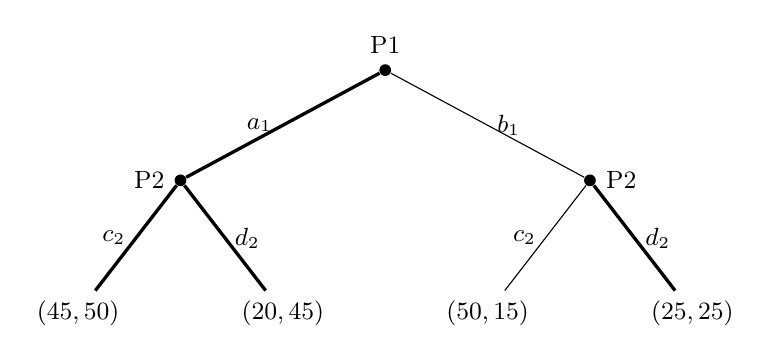
\begin{tikzpicture}[level distance=14mm, level 1/.style={sibling distance=52mm},
  level 2/.style={sibling distance=26mm}, every node/.style={font=\small}]
\node[dec,label=above:{P1}]{}
  child{node[dec,label=left:{P2}]{}
    child{node[below]{$(45,50)$} edge from parent[very thick] node[left]{$c_2$}}
    child{node[below]{$(20,45)$} edge from parent node[right]{$d_2$}}
    edge from parent[very thick] node[left]{$a_1$}}
  child{node[dec,label=right:{P2}]{}
    child{node[below]{$(50,15)$} edge from parent node[left]{$c_2$}}
    child{node[below]{$(25,25)$} edge from parent[very thick] node[right]{$d_2$}}
    edge from parent node[right]{$b_1$}};
\end{tikzpicture}\\
\small Thick lines are the backward-induction choices.
\end{center}

\subsection{Solution concepts}
\begin{defbox}{Definitions}
\begin{itemize}
\item \textbf{Strictly dominated:} $s_i$ is strictly dominated by $s_i'$ if $u_i(s_i',s_{-i})>u_i(s_i,s_{-i})$ for \emph{every} $s_{-i}$.
\item \textbf{Strictly dominant:} $s_i^*$ strictly dominates every other strategy in $S_i$.
\item \textbf{IDSDS:} start from $S_i$ and repeatedly delete strategies that are strictly dominated given the strategies \emph{still remaining} for the others.
\item \textbf{Rationalizable:} survives repeated removal of strategies that are not a best response to \emph{any} belief about the others' remaining strategies.
\item \textbf{Best response:} $BR_i(s_{-i})=\arg\max_{s_i\in S_i}u_i(s_i,s_{-i})$.
\item \textbf{Nash equilibrium:} $s^*$ such that $s_i^*\in BR_i(s_{-i}^*)$ for every $i$. Equivalently, $u_i(s_i^*,s_{-i}^*)\ge u_i(s_i,s_{-i}^*)$ for all $s_i$ and all $i$: no profitable \emph{unilateral} deviation.
\item \textbf{SPE:} a NE that also induces a NE in every subgame. In finite games of perfect information, use backward induction.
\end{itemize}
\end{defbox}

\textbf{The hierarchy (what each assumes):}
\begin{center}
\begin{tabular}{@{}p{3.6cm}p{5.4cm}p{5.6cm}@{}}
\toprule
Concept & Assumes & Use\\\midrule
Dominant strategies & rationality only & design games so everyone has one (robust)\\
IDSDS / rationalizability & $+$ common knowledge of rationality & ``RAT brutal'': weak predictions\\
Nash equilibrium & $+$ correct beliefs about others' play & sharp; ``NE easy''\\
\bottomrule
\end{tabular}
\end{center}
\textbf{NE always sits inside the set of rationalizable outcomes} (NE $\subseteq$ survivors of IDSDS). The reverse does not hold.

\begin{tipbox}
\begin{itemize}[nosep]
\item Only \textbf{strict} dominance deletes. If two strategies tie in any column, it is not strict, so do not delete. Sequential-game matrices are full of ties, because P2's plan at an unreached node does not change the payoff.
\item To find pure NE: underline each player's best response in every row/column. Cells with both underlined are the NE.
\item NE of a sequential game that are \emph{not} SPE rest on \textbf{incredible threats} (a plan P2 would never carry out at that node).
\end{itemize}
\end{tipbox}

\begin{workbox}{PS2 \#1: IDSDS and NE (Greg rows, Phil columns)}
\begin{center}
\begin{tabular}{c|ccc}
 & $n_P$ & $l_P$ & $h_P$\\\hline
$n_G$ & 0, 0 & 1, 2 & 1, 2\\
$l_G$ & 3, 1 & 3, 3 & 3, 4\\
$h_G$ & 2, 1 & 4, 3 & 5, 5
\end{tabular}
\end{center}
Delete $n_G$ (dominated by $l_G$: $3>0,3>1,3>1$). Then delete $n_P$ (dominated by $l_P$: $3>1,3>1$). Then delete $l_G$ (dominated by $h_G$: $4>3,5>3$). Then delete $l_P$ (dominated by $h_P$: $5>3$). Survivor: $(h_G,h_P)$, which is also the unique NE.
\end{workbox}

\begin{workbox}{PS2 \#2: a 2$\times$3 sequential game (P2 has 9 strategies)}
P1 picks $a_1/b_1$, then P2 observes and picks $c_2/d_2/e_2$. The payoffs are
$(a,c)=(10,8)$, $(a,d)=(8,9)$, $(a,e)=(12,11)$, $(b,c)=(13,0)$, $(b,d)=(1,10)$, $(b,e)=(10,6)$.

$S_2=\{cc,cd,ce,dc,dd,de,ec,ed,ee\}$ (first letter after $a_1$, second after $b_1$).\\
P2's best responses: vs $a_1$, any strategy starting with $e$; vs $b_1$, any strategy ending in $d$.\\
NE with $a_1$: P2 $\in\{ec,ed,ee\}$, and P1 must prefer $a_1$ (12) to $b_1$. Against $ec$, $b_1$ gives 13, so that fails. Against $ed$ ($b_1$ gives 1) and $ee$ ($b_1$ gives 10) it works.\\
NE with $b_1$: P2 $\in\{cd,dd,ed\}$, and $b_1$ gives 1, which is worse than $a_1$ every time. None.\\
$NE=\{(a_1,ed),(a_1,ee)\}$. Backward induction: $e$ after $a_1$, $d$ after $b_1$, P1 picks $a_1$. $SPE=(a_1,ed)$.\\
$(a_1,ee)$ uses an incredible threat: $e$ after $b_1$, where P2 would really pick $d$ ($10>6$).\\
\small(The printed official key for this question reads ``$(b;ec)$'', which looks garbled. Check that the logic above matches your own.)
\end{workbox}

\subsection{Mixed strategies}
\begin{defbox}{Mixed strategies}
A \textbf{mixed strategy} $\sigma_i\in\Delta(S_i)$ is a probability distribution over pure strategies. A \textbf{mixed NE} is $\sigma^*$ with $U_i(\sigma_i^*,\sigma_{-i}^*)\ge U_i(\sigma_i,\sigma_{-i}^*)$ for all $\sigma_i$ and all $i$. \textbf{Every finite game has at least one NE in mixed strategies.}
\end{defbox}
\textbf{Recipe (the indifference trick):} if a player mixes, she must be \emph{indifferent} between the pure strategies she uses. So choose \emph{my} probability to make \emph{the other player} indifferent.

\textbf{Matching pennies:} P1 wins on a match. With $q=\Pr(\text{P2 plays }H)$: $U_1(H)=2q-1$ and $U_1(T)=1-2q$, so indifference gives $q=1/2$. By symmetry $p=1/2$. The mixed NE is $(1/2,1/2)$.


\subsection{Expected exam questions}
\begin{examq}{a full sequential game}
Player 1 chooses $a_1$ or $b_1$. Player 2 observes the choice, then chooses $c_2$ or $d_2$. Payoffs: $u_1(a_1,c_2)=30$, $u_2=10$; $u_1(a_1,d_2)=0$, $u_2=20$; $u_1(b_1,c_2)=20$, $u_2=30$; $u_1(b_1,d_2)=10$, $u_2=25$.\\
(a) Write the normal form. (b) Construct the game matrix. (c) Find the strategies that survive IDSDS. (d) Find all NE. (e) Draw the tree and find all SPE.
\soln
(a) $N=\{1,2\}$, $S_1=\{a_1,b_1\}$, $S_2=\{c_2c_2,c_2d_2,d_2c_2,d_2d_2\}$ (first letter after $a_1$, second after $b_1$). Payoffs $u_i(s_1,s_2)$ are those at the terminal node reached.

(b)
\begin{center}
\begin{tabular}{c|cccc}
 & $c_2c_2$ & $c_2d_2$ & $d_2c_2$ & $d_2d_2$\\\hline
$a_1$ & 30, 10 & 30, 10 & 0, 20 & 0, 20\\
$b_1$ & 20, 30 & 10, 25 & 20, 30 & 10, 25
\end{tabular}
\end{center}
(c) P1: $a_1=(30,30,0,0)$ and $b_1=(20,10,20,10)$, so there is no dominance. P2's payoffs against $(a_1,b_1)$: $c_2c_2=(10,30)$, $c_2d_2=(10,25)$, $d_2c_2=(20,30)$, $d_2d_2=(20,25)$. $d_2c_2$ \emph{strictly} dominates $c_2d_2$ ($20>10$, $30>25$), so delete $c_2d_2$. Every other comparison has a tie. Next round, P1 against the remaining columns: $a_1=(30,0,0)$ and $b_1=(20,20,10)$, still no dominance. Survivors: $\{a_1,b_1\}\times\{c_2c_2,d_2c_2,d_2d_2\}$.

(d) P1 best responses: $a_1,a_1,b_1,b_1$. P2 best responses: vs $a_1$, $\{d_2c_2,d_2d_2\}$; vs $b_1$, $\{c_2c_2,d_2c_2\}$. The only cell where both are best responding is $(b_1,d_2c_2)$, so $NE=\{(b_1,d_2c_2)\}$.

(e) After $a_1$, P2 plays $d_2$ ($20>10$); after $b_1$, P2 plays $c_2$ ($30>25$). P1 compares $0$ with $20$ and plays $b_1$. $SPE=\{(b_1,d_2c_2)\}$, with outcome $(20,30)$.\\
\emph{Lesson:} IDSDS left six cells, but NE picks out one. NE $\subseteq$ rationalizable, and NE is much sharper.
\end{examq}

\begin{examq}{simultaneous vs.\ sequential normal forms (PS2 \#3 style)}
Each player picks 0 or 1. Player 1 gets \$1 if the actions match and \$0 otherwise. Player 2 gets \$1 if they don't match and \$0 otherwise. Players care only about their own money.
(a) Give the normal form if the game is simultaneous. (b) Give the normal form if Player 1 moves first and Player 2 observes. (c) Find the SPE of (b). (d) What is the only difference between the two normal forms?
\soln
(a) $N=\{1,2\}$, $S_1=S_2=\{0,1\}$. Payoffs: $(1,0)$ on a match and $(0,1)$ on a mismatch. This is matching pennies: there is no pure NE, and the mixed NE has each player play 0 with probability $\tfrac12$.

(b) $S_1=\{0,1\}$ and $S_2=\{00,01,10,11\}$ ($xy$: $x$ after 0, $y$ after 1).
\begin{center}
\begin{tabular}{c|cccc}
 & $00$ & $01$ & $10$ & $11$\\\hline
$0$ & 1, 0 & 1, 0 & 0, 1 & 0, 1\\
$1$ & 0, 1 & 1, 0 & 0, 1 & 1, 0
\end{tabular}
\end{center}
(c) P2 always mismatches: 1 after 0 and 0 after 1, which is the strategy $10$. P1 then gets 0 whatever she does, so she is indifferent. $SPE=\{(0,10),(1,10)\}$. The second mover wins.

(d) Players and payoffs over outcomes are the same. Only the \textbf{strategy sets} differ: observing P1's move turns P2's 2 actions into 4 contingent plans.
\end{examq}

\begin{examq}{mixed strategy NE}
Find all Nash equilibria (pure and mixed) of
\[
\begin{array}{c|cc}
 & L & R\\\hline
U & 3,1 & 0,0\\
D & 0,0 & 1,3
\end{array}
\]
\soln
\emph{Pure:} $(U,L)$ has P1 at $3>0$ and P2 at $1>0$, so neither deviates: NE. $(D,R)$ has $1>0$ and $3>0$: NE. $(U,R)$ and $(D,L)$ are not NE.

\emph{Mixed:} let $p=\Pr(U)$ and $q=\Pr(L)$. To make P2 indifferent: $1\cdot p=3(1-p)\Rightarrow p=\tfrac34$. To make P1 indifferent: $3q=1\cdot(1-q)\Rightarrow q=\tfrac14$.

So there are \textbf{three NE}: $(U,L)$, $(D,R)$ and $\big((\tfrac34U,\tfrac14D),(\tfrac14L,\tfrac34R)\big)$. In the mixed NE each player expects $\tfrac34$, which is worse for both than either pure NE: another case where NE is not efficient.
\end{examq}

%=====================================================================
\section{Games where money is not the payoff}
This is last year's Section 2.2 format, and PS2 \#4 is the idea behind it.

\textbf{The key point:} the money matrix is \emph{not} the game matrix. Payoffs come from \emph{preferences}. Before solving, convert money into each player's utility for each case.

\begin{workbox}{Last year's money game: $(R,R)=\$9,\$9$; $(R,Q)=\$0,\$20$; $(Q,R)=\$20,\$0$; $(Q,Q)=\$2,\$2$; sequential}
\textbf{Case 1 (selfish):} after $R_1$, P2 plays $Q$ ($20>9$); after $Q_1$, P2 plays $Q$ ($2>0$). P1 gets $0$ from $R$ and $2$ from $Q$, so she plays $Q$. $SPE=(Q_1,Q_2Q_2)$ with outcome $(\$2,\$2)$, a Prisoner's Dilemma. NE: in the $2\times4$ matrix, only $(Q_1,Q_2Q_2)$.

\textbf{Case 2 (each maximizes the total):} totals are $RR=18$, $RQ=20$, $QR=20$, $QQ=4$. After $R_1$, P2 plays $Q$ ($20>18$); after $Q_1$, P2 plays $R$ ($20>4$). P1 is indifferent ($20=20$). SPE: $(R_1,Q_2R_2)$ and $(Q_1,Q_2R_2)$.

\textbf{Case 3 (Nature picks 2a with probability $\mu$ or 2b; P1 cares about her money $+$ 2b's):} vs 2a (selfish), 2a plays $Q$ always, so P1 gets $0$ after $R_1$ and $2$ after $Q_1$. vs 2b (cares about the sum with P1), P1's payoff is the total: $20$ after either action. $E[R_1]=20(1-\mu)$ and $E[Q_1]=2\mu+20(1-\mu)$, so \textbf{$Q_1$ is strictly better for every $\mu\in(0,1)$}.\\
\emph{Difficulties to mention:} P1 doesn't know which subgame she is in (imperfect information), so we need a Nature move, an information set, beliefs $\mu$ and expected payoffs. That goes beyond plain backward induction.
\end{workbox}

\textbf{PS2 \#4 lesson (``third-party observation''):} seeing everyone play $M$ in a money game does \emph{not} reject game theory or rationality. We don't know players' preferences over money, so we can always build payoffs that make $(M_1,M_2)$ the unique NE. To test rationality you need to know preferences.


\subsection*{Expected exam question}
\begin{examq}{money game with an \emph{equity} case}
The money each player gets (this is \emph{not} the game matrix): $(R_1,R_2)=\$5,\$5$; $(R_1,Q_2)=\$1,\$8$; $(Q_1,R_2)=\$8,\$1$; $(Q_1,Q_2)=\$3,\$3$. Player 1 moves first, and Player 2 observes and then moves.\\
\emph{Case 1:} each player cares only about his or her own money.
\emph{Case 2:} each player cares only about the \emph{smaller} of the two players' money amounts (a Rawlsian concern for equity).\\
For each case, write the game matrix, find all NE and find the SPE.
\soln
$S_1=\{R_1,Q_1\}$ and $S_2=\{R_2R_2,R_2Q_2,Q_2R_2,Q_2Q_2\}$ (after $R_1$, after $Q_1$).

\textbf{Case 1:}
\begin{center}
\begin{tabular}{c|cccc}
 & $R_2R_2$ & $R_2Q_2$ & $Q_2R_2$ & $Q_2Q_2$\\\hline
$R_1$ & 5, 5 & 5, 5 & 1, 8 & 1, 8\\
$Q_1$ & 8, 1 & 3, 3 & 8, 1 & 3, 3
\end{tabular}
\end{center}
P1 best responses: $Q_1,R_1,Q_1,Q_1$. P2 best responses: vs $R_1$, $\{Q_2R_2,Q_2Q_2\}$; vs $Q_1$, $\{R_2Q_2,Q_2Q_2\}$. $NE=\{(Q_1,Q_2Q_2)\}$. Backward induction: P2 plays $Q_2$ after both actions, and P1 compares $1$ with $3$ and plays $Q_1$. $SPE=(Q_1,Q_2Q_2)$, with outcome $(\$3,\$3)$, Pareto dominated by $(\$5,\$5)$.

\textbf{Case 2:} both payoffs are $\min$ of the money: $RR\to5$, $RQ\to1$, $QR\to1$, $QQ\to3$.
\begin{center}
\begin{tabular}{c|cccc}
 & $R_2R_2$ & $R_2Q_2$ & $Q_2R_2$ & $Q_2Q_2$\\\hline
$R_1$ & 5, 5 & 5, 5 & 1, 1 & 1, 1\\
$Q_1$ & 1, 1 & 3, 3 & 1, 1 & 3, 3
\end{tabular}
\end{center}
P1 best responses: $R_1$, $R_1$, $\{R_1,Q_1\}$, $Q_1$. P2 best responses: vs $R_1$, $\{R_2R_2,R_2Q_2\}$; vs $Q_1$, $\{R_2Q_2,Q_2Q_2\}$. $NE=\{(R_1,R_2R_2),(R_1,R_2Q_2),(Q_1,Q_2Q_2)\}$. Backward induction: after $R_1$, $R_2$ ($5>1$); after $Q_1$, $Q_2$ ($3>1$). P1 plays $R_1$. $SPE=(R_1,R_2Q_2)$, with outcome $(\$5,\$5)$.\\
\emph{Lesson:} the money is the same, but different preferences give a different game. $(Q_1,Q_2Q_2)$ is a NE only because of the incredible threat to play $Q_2$ after $R_1$.
\end{examq}

%=====================================================================
\section{Cournot oligopoly from scratch (75 min with \S6)}

\subsection{The story}
Firms produce a \textbf{homogeneous} good and \textbf{choose quantities} at the same time. Total output $Q$ then hits the market, and the price adjusts to clear it: $p=P(Q)$. Think of bottled-water suppliers who must commit to output before they know the price. Each firm's best quantity depends on what the others produce, which makes it a game.

\textbf{Notation:} $q_i$ is firm $i$'s output, $Q=\sum_j q_j$, and $Q_{-i}=Q-q_i$ is everyone else's output. Inverse demand is $P(Q)$ and the cost is $C_i(q_i)$.

\subsection{Normal form of a Cournot game (say this every time)}
\[
N=\{1,\dots,n\},\qquad S_i=[0,\bar q]\ (\text{quantities}),\qquad
\pi_i(q_i,Q_{-i})=\underbrace{P(q_i+Q_{-i})\,q_i}_{\text{revenue}}-\underbrace{C_i(q_i)}_{\text{cost}}.
\]

\subsection{Calculus you need (only this)}
\begin{itemize}
\item $\dfrac{d}{dq}(aq)=a$, $\ \dfrac{d}{dq}(q^2)=2q$, $\ \dfrac{d}{dq}\big(\tfrac c2q^2\big)=cq$. Anything that doesn't contain $q_i$ (like $Q_{-i}$) is a \emph{constant} when you differentiate with respect to $q_i$.
\item \textbf{FOC:} set $\partial\pi_i/\partial q_i=0$ and solve for $q_i$.
\item \textbf{SOC:} $\partial^2\pi_i/\partial q_i^2<0$ means profit is concave, so the FOC gives a maximum. With linear demand and linear or quadratic costs it always holds; say so in one line.
\end{itemize}

\subsection{The 4-step recipe}
\begin{workbox}{Solving any Cournot game}
\begin{enumerate}[label=\textbf{Step \arabic*.},leftmargin=4.2em]
\item \textbf{Profit.} Write $\pi_i=(a-q_i-Q_{-i})q_i-C(q_i)$ \emph{before} imposing anything.
\item \textbf{Best response.} Differentiate with respect to $q_i$ only, set it to 0, and solve: $q_i=b_i(Q_{-i})$. It slopes down, because quantities are \emph{strategic substitutes}. Truncate at 0 if negative.
\item \textbf{Equilibrium.} NE means every firm is on its BR at once. With identical firms, \emph{now} impose symmetry: $q_i=q^c$ and $Q_{-i}=(n-1)q^c$, and solve the single equation. With different firms, solve the BR equations together.
\item \textbf{Everything else.} $Q^c=nq^c$, $p^c=P(Q^c)$, $\pi_i$, CS, PS, TS, the efficient outcome, DWL, and the graph.
\end{enumerate}
\end{workbox}
\begin{tipbox}
The notes' \#1 mistake: \textbf{do not set $q_1=q_2$ before differentiating.} A firm controls only its own $q_i$ and takes $Q_{-i}$ as given. Impose symmetry only in Step 3. Second mistake: treating $Q$ as if one firm controls all of it.
\end{tipbox}

\subsection{Worked: the lecture example (from your 10/22 notes)}
$P(Q)=100-Q$, $c(q_i)=10q_i$, $n=3$.
\begin{enumerate}
\item $\pi_i=(100-q_i-Q_{-i})q_i-10q_i$.
\item FOC: $100-2q_i-Q_{-i}-10=0\Rightarrow b_i(Q_{-i})=\dfrac{90-Q_{-i}}{2}$.
\item Symmetry, $Q_{-i}=2q^c$: $q^c=\dfrac{90-2q^c}{2}\Rightarrow4q^c=90\Rightarrow q^c=22.5$.
\item $Q^c=67.5$, $p^c=32.5$, $\pi_i=(32.5-10)(22.5)=506.25$. Efficient: $p=MC=10\Rightarrow Q^*=90$. $CS=\tfrac12(67.5)^2=2278.1$, $PS=1518.75$, $DWL=\tfrac12(90-67.5)(32.5-10)=253.1$.
\end{enumerate}
(Your notes wrote ``$q^c=90/4$''; that is exactly $22.5$. Notes check: correct.)

\subsection{Welfare: what to compute and draw}
\begin{defbox}{Welfare definitions}
\begin{itemize}
\item \textbf{Consumer surplus} $CS$: the area under demand and above $p^c$, up to $Q^c$. With $P=a-Q$ it is $\tfrac12Q^c(a-p^c)=\tfrac12(Q^c)^2$.
\item \textbf{Producer surplus} $PS$: the area above MC and below $p^c$, up to $Q^c$. With no fixed costs, $PS=\sum_i\pi_i$.
\item \textbf{Total surplus} $TS=CS+PS$, the total gains from trade.
\item \textbf{Efficient outcome:} maximize TS, i.e.\ produce until $P(Q)=MC$, using the cheapest producers. If each firm has rising MC, split output so their MCs are equal.
\item \textbf{Deadweight loss} $DWL=TS^*-TS^c$: the surplus lost from trades worth more to buyers than they cost to make that don't happen. Graphically, the triangle between demand and MC from $Q^c$ to $Q^*$.
\end{itemize}
\end{defbox}

\textbf{Why Cournot is inefficient:} when firm $i$ expands, the price falls on \emph{all} units, including rivals'. Firm $i$ counts only its own loss ($P'(Q)q_i$), so each firm restricts output to keep the price up, the market \textbf{underproduces}, and $p>MC$. This is a NE that is not Pareto efficient, just like the Prisoner's Dilemma. Firms ``make more gains from trade themselves'' by selling less at a high price.

\textbf{Benchmarks to remember} (linear demand $a-bQ$, constant MC $c$): $q^c=\dfrac{a-c}{(n+1)b}$, $p^c=\dfrac{a+nc}{n+1}$. $n=1$ is monopoly; as $n\to\infty$, $p\to c$ (competitive). Ordering: $Q^m<Q^c_2<Q^c_3<\dots<Q^{PC}$ and $p^m>p^c_2>\dots>MC$. The Cournot markup is $\dfrac{p-MC_i}{p}=\dfrac{s_i}{|\varepsilon_D|}$ (a bigger market share or less elastic demand means a bigger markup).


\subsection*{Expected exam question}
\begin{examq}{Cournot duopoly with constant marginal cost}
Two firms choose quantities simultaneously. $P(Q)=150-Q$ and $C(q_i)=30q_i$.
(a) Write the normal form. (b) Find firm $i$'s best response. (c) Find $q^c$, $Q^c$, $p^c$. (d) Find each firm's profit and CS, PS, TS. (e) Find the efficient outcome and the DWL, and draw the $p$--$Q$ graph. (f) Compare with a monopolist that has the same costs, and explain the ranking.
\soln
(a) $N=\{1,2\}$, $S_i=[0,150]$, $\pi_i(q_i,q_j)=(150-q_i-q_j)q_i-30q_i$.

(b) FOC: $150-2q_i-q_j-30=0\Rightarrow b_i(q_j)=\dfrac{120-q_j}{2}$. SOC: $-2<0$.

(c) With symmetry \emph{after} the FOC: $q=\tfrac{120-q}{2}\Rightarrow3q=120\Rightarrow q^c=40$, $Q^c=80$, $p^c=70$.

(d) $\pi_i=(70-30)(40)=1600$. $PS=3200$. $CS=\tfrac12(80)(150-70)=3200$. $TS=6400$.

(e) Efficient: $p=MC=30\Rightarrow Q^*=120$, $TS^*=\tfrac12(120)(120)=7200$. $DWL=800=\tfrac12(120-80)(70-30)$. On the graph: demand runs from $(0,150)$ to $(150,0)$, MC is flat at $30$, CS the triangle above $p=70$, PS the rectangle from $30$ to $70$ over $[0,80]$, and DWL the triangle from $Q=80$ to $120$.

(f) Monopoly: $\max(150-Q)Q-30Q\Rightarrow Q^m=60$, $p^m=90$, $\pi^m=3600$, $CS=1800$, $TS=5400$, $DWL=1800$. So $Q^m=60<Q^c=80<Q^*=120$ and $p^m>p^c>MC$. With two firms, each one ignores how its extra output lowers the \emph{rival's} revenue, so together they produce more than a monopolist. That is still less than efficient, because each firm still counts the price drop on its \emph{own} units.
\end{examq}

%=====================================================================
\section{Problem Set 3, fully solved (Cournot parts)}
Try each part yourself first, then check. PS3 \#4 is Bertrand, which the professor said is not on the midterm, so it is skipped here.

\subsection*{PS3 \#1: Cournot duopoly, $P(Q)=200-Q$, $C(q_i)=cq_i^2/2$}
\textbf{1.a Profit.} $\pi_i=(200-q_i-q_j)q_i-\dfrac c2q_i^2$.

\textbf{1.b Best response.} $\dfrac{\partial\pi_i}{\partial q_i}=200-2q_i-q_j-cq_i=0\Rightarrow\boxed{b_i(q_j)=\dfrac{200-q_j}{2+c}}$. SOC: $-(2+c)<0$.\\
Graph: $b_1$ hits the $q_1$-axis at $200/(2+c)$ and the $q_2$-axis at $200$. $b_2$ is its mirror image. They cross on the 45$^\circ$ line.

\begin{center}
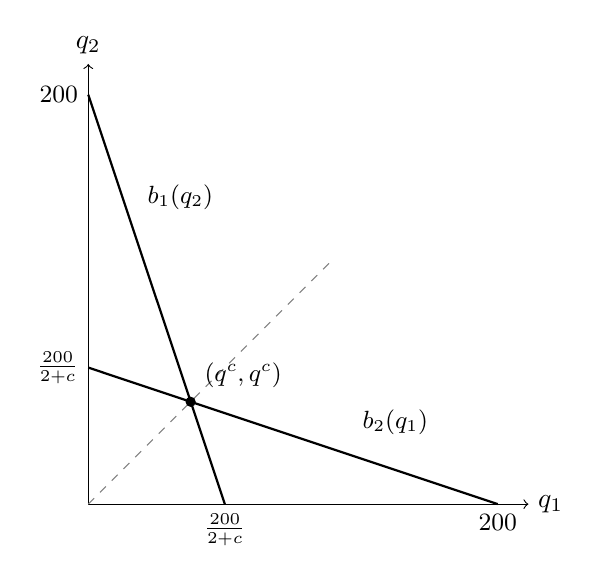
\begin{tikzpicture}[scale=0.026]
\draw[->] (0,0)--(215,0) node[right]{$q_1$};
\draw[->] (0,0)--(0,215) node[above]{$q_2$};
\draw[thick] (66.7,0)--(0,200) node[left]{\small 200};
\draw[thick] (0,66.7)--(200,0) node[below]{\small 200};
\node[below] at (66.7,0){\small $\frac{200}{2+c}$};
\node[left] at (0,66.7){\small $\frac{200}{2+c}$};
\node at (45,150){\small $b_1(q_2)$};
\node at (150,40){\small $b_2(q_1)$};
\draw[dashed,gray] (0,0)--(120,120);
\fill (50,50) circle (2.5);
\node[above right] at (52,52){\small $(q^c,q^c)$};
\end{tikzpicture}\\
\small Drawn for $c=1$: the intercepts are $66.7$ and the equilibrium is $(50,50)$.
\end{center}

\textbf{1.c Equilibrium.} With symmetry,
\[(2+c)q=200-q\ \Rightarrow\ \boxed{q^c=\dfrac{200}{3+c}},\qquad Q^c=\dfrac{400}{3+c},\qquad \boxed{p^c=200-\dfrac{400}{3+c}=\dfrac{200(1+c)}{3+c}}.\]

\textbf{1.d Graph on the $p$--$Q$ plane.} Demand $P=200-Q$. The industry MC curve: each firm has $MC=cq_i$, and with output split evenly ($q_i=Q/2$), $MC(Q)=\tfrac c2Q$. Mark $(Q^c,p^c)$ on demand, the efficient point where demand crosses $MC(Q)$, and shade CS, PS, DWL.

\begin{center}
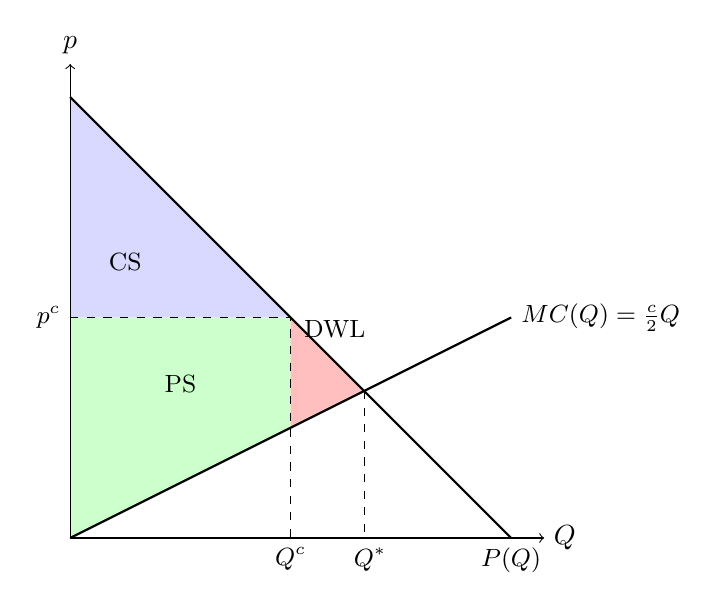
\begin{tikzpicture}[scale=0.028]
\fill[blue!15] (0,200)--(0,100)--(100,100)--cycle;
\fill[green!20] (0,0)--(0,100)--(100,100)--(100,50)--cycle;
\fill[red!25] (100,100)--(100,50)--(133.3,66.7)--cycle;
\draw[->] (0,0)--(215,0) node[right]{$Q$};
\draw[->] (0,0)--(0,215) node[above]{$p$};
\draw[thick] (0,200)--(200,0) node[below]{\small $P(Q)$};
\draw[thick] (0,0)--(200,100) node[right]{\small $MC(Q)=\tfrac c2Q$};
\draw[dashed] (0,100)--(100,100)--(100,0);
\draw[dashed] (133.3,66.7)--(133.3,0);
\node[left] at (0,100){\small $p^c$};
\node[below] at (100,0){\small $Q^c$};
\node[below] at (136,0){\small $Q^*$};
\node at (25,125){\small CS};
\node at (50,70){\small PS};
\node at (120,95){\small DWL};
\end{tikzpicture}\\
\small Drawn for $c=1$: $Q^c=100$, $p^c=100$, $Q^*=133.3$, $p^*=66.7$.
\end{center}

\textbf{1.e Profits and welfare.}
\begin{align*}
\pi_i&=p^cq^c-\tfrac c2(q^c)^2=q^c\Big(p^c-\tfrac c2q^c\Big)=\frac{200}{3+c}\cdot\frac{200(1+c)-100c}{3+c}=\boxed{\frac{20000(2+c)}{(3+c)^2}}\\
CS&=\tfrac12Q^c(200-p^c)=\tfrac12(Q^c)^2=\boxed{\frac{80000}{(3+c)^2}},\qquad PS=2\pi_i=\frac{40000(2+c)}{(3+c)^2}\\
TS&=CS+PS=\boxed{\frac{40000(4+c)}{(3+c)^2}}
\end{align*}
\emph{Efficient:} $200-Q=\tfrac c2Q\Rightarrow Q^*=\dfrac{400}{2+c}$ and $p^*=\dfrac{200c}{2+c}$, so
\[TS^*=200Q^*-\tfrac12(Q^*)^2-2\cdot\tfrac c2\Big(\tfrac{Q^*}{2}\Big)^2=\frac{40000}{2+c},\qquad
\boxed{DWL=TS^*-TS=\frac{40000}{(2+c)(3+c)^2}}.\]
\emph{Check with $c=1$:} $q^c=50$, $p^c=100$, $\pi_i=3750$, $CS=5000$, $TS=12{,}500$, $TS^*=13{,}333$, $DWL=833$. These match the Ch.~5 notes.

\subsection*{PS3 \#2: the same model with $n$ firms}
\textbf{2.a} $\pi_i=(200-q_i-Q_{-i})q_i-\dfrac c2q_i^2$.

\textbf{2.b} FOC: $200-2q_i-Q_{-i}-cq_i=0\Rightarrow\boxed{b_i(Q_{-i})=\dfrac{200-Q_{-i}}{2+c}}$. On the $q_i$--$Q_{-i}$ plane this is a line from $q_i=\frac{200}{2+c}$ (at $Q_{-i}=0$) down to $Q_{-i}=200$.

\textbf{2.c} Symmetry, $Q_{-i}=(n-1)q$: $(2+c)q=200-(n-1)q\Rightarrow\boxed{q^c=\dfrac{200}{n+1+c}}$, $Q^c=\dfrac{200n}{n+1+c}$, $\boxed{p^c=\dfrac{200(1+c)}{n+1+c}}$.

\textbf{2.d} Same picture as 1.d, with the industry MC now $MC(Q)=\frac cnQ$ (output split $n$ ways), which gets flatter as $n$ grows.

\textbf{2.e}
\begin{align*}
\pi_i&=\Big(1+\frac c2\Big)\Big(\frac{200}{n+1+c}\Big)^2=\frac{20000(2+c)}{(n+1+c)^2},\qquad
CS=\tfrac12(Q^c)^2=\frac{20000\,n^2}{(n+1+c)^2},\\
PS&=n\pi_i=\frac{20000\,n(2+c)}{(n+1+c)^2},\qquad
TS=\frac{20000\,n(n+2+c)}{(n+1+c)^2}.
\end{align*}
Efficient: $200-Q=\frac cnQ\Rightarrow Q^*=\dfrac{200n}{n+c}$, $TS^*=\dfrac{20000\,n}{n+c}$, so
\[\boxed{DWL=\frac{20000\,n}{(n+c)(n+1+c)^2}}\ \xrightarrow[n\to\infty]{}\ 0.\]
(For $n=2$ this reduces to the 1.e formulas, which is a good self-check.) \textbf{Interpretation:} more firms means each firm has less effect on price, so the underproduction shrinks and $p^c$ approaches MC. With rising MC, more firms also spread production, which lowers the cost of any given $Q$.

\subsection*{PS3 \#3: differentiated products, $P_1=18-q_1-\gamma q_2$, $P_2=18-q_2-\gamma q_1$, no costs, $\gamma\in(0,1)$}
$\gamma$ measures how substitutable the goods are: $\gamma=0$ means independent goods, $\gamma=1$ means identical goods.
\begin{itemize}
\item \textbf{3.a} $\pi_1=(18-q_1-\gamma q_2)q_1$ and $\pi_2=(18-q_2-\gamma q_1)q_2$.
\item \textbf{3.b} FOC: $18-2q_1-\gamma q_2=0\Rightarrow b_1(q_2)=\dfrac{18-\gamma q_2}{2}$; symmetrically $b_2(q_1)=\dfrac{18-\gamma q_1}{2}$.
\item \textbf{3.c} Each BR is a line from $9$ on its own axis down to $18/\gamma$ on the other axis. A smaller $\gamma$ makes the lines flatter (less strategic interaction).
\item \textbf{3.d} Symmetry: $2q=18-\gamma q\Rightarrow\boxed{q_i(\gamma)=\dfrac{18}{2+\gamma}}$ and $p_i(\gamma)=18-(1+\gamma)\dfrac{18}{2+\gamma}=\boxed{\dfrac{18}{2+\gamma}}$. Profit is $\big(\tfrac{18}{2+\gamma}\big)^2$.\\
At $\gamma=0$ we get two monopolies ($q=p=9$); at $\gamma=1$, homogeneous Cournot ($q=p=6$). More differentiation (a lower $\gamma$) gives a higher price and profit, because there is less competition.
\end{itemize}


\subsection*{Expected exam questions}
\begin{examq}{PS3 \#2 with numbers}
In PS3 \#2 ($P=200-Q$, $C(q_i)=cq_i^2/2$, $n$ firms), let $c=1$ and $n=4$. Find $b_i(Q_{-i})$, $q^c$, $p^c$, each firm's profit, CS, TS and DWL. How does the DWL compare with the duopoly ($n=2$)?
\soln
$\pi_i=(200-q_i-Q_{-i})q_i-\tfrac12q_i^2$. The FOC $200-3q_i-Q_{-i}=0$ gives $b_i(Q_{-i})=\dfrac{200-Q_{-i}}{3}$.\\
With symmetry, $Q_{-i}=3q$: $3q=200-3q\Rightarrow q^c=\tfrac{200}{6}=33.3$, $Q^c=133.3$, $p^c=66.7$.\\
$\pi_i=p^cq^c-\tfrac12(q^c)^2=2222.2-555.6=1666.7$. $CS=\tfrac12(Q^c)^2=8888.9$. $PS=4\pi_i=6666.7$. $TS=15{,}555.6$.\\
Efficient: $MC_i=q_i=Q/4$, so $200-Q=Q/4\Rightarrow Q^*=160$, $p^*=40$, $TS^*=16{,}000$. $DWL=444.4$.\\
With $n=2$, $DWL=833.3$. Doubling the number of firms roughly halves the loss: more competition means less underproduction.
\end{examq}

\begin{examq}{product differentiation (PS3 \#3)}
In PS3 \#3, equilibrium is $q_i=p_i=\dfrac{18}{2+\gamma}$. How do quantities, prices and profits change as $\gamma$ rises from 0 to 1? Interpret.
\soln
All three fall as $\gamma$ rises: from $q=p=9$ and $\pi=81$ at $\gamma=0$ to $q=p=6$ and $\pi=36$ at $\gamma=1$. $\gamma$ measures how close substitutes the goods are. At $\gamma=0$, each firm is a monopolist in its own market. As $\gamma\to1$, a rival's output cuts into my price more, so competition is fiercer and we approach homogeneous Cournot. Differentiation softens competition and protects markups.
\end{examq}

%=====================================================================
\section{Market games, efficiency and equity (15 min)}

\begin{defbox}{Definitions from the notes}
\begin{itemize}
\item \textbf{Pareto efficient:} there is no way to change production or allocation to make someone better off without hurting anyone else.
\item \textbf{Productive efficiency:} production happens at minimum cost (you can't make more of one thing without less of another).
\item \textbf{Allocative efficiency:} each good goes to the person who values it most.
\item \textbf{Equity:} fairness, which can be defined in many ways. It needs a separate normative criterion.
\end{itemize}
\end{defbox}

\textbf{Points to be able to make:}
\begin{enumerate}
\item \textbf{NE is generally neither efficient nor equitable.} The Prisoner's Dilemma shows inefficiency. Equity is not even part of the definition of NE.
\item \textbf{Market games have natural welfare measures:} gains from trade for each person. Buyers get $CS=WTP-p$ and sellers get $PS=p-WTS$. $TS=CS+PS$ is the starting point for evaluation. It measures efficiency, \emph{not} equity, because it ignores who gets the surplus.
\item \textbf{Pure exchange (no production):} trade is voluntary, so every trade is mutually beneficial. NE does not need perfect competition, and gains from trade are maximized as long as there are no \emph{transaction costs}. Crime and scams (information problems) are what get in the way.
\item \textbf{Adding production} raises two questions: (1) \emph{what} each firm produces (which firms should produce) and (2) \emph{how much} each firm produces (the course focuses on this, using partial equilibrium for one industry). Oligopolies \textbf{underproduce} to raise price, and sometimes \textbf{the wrong (high-cost) firms produce}.
\item \textbf{Asymmetric-cost Cournot example} ($P=120-Q$, $c_1=20$, $c_2=40$): $q_1=40$, $q_2=20$, $p=60$. Efficiently, firm 1 would make all $100$ units at $p=20$. $DWL=1200=800$ (underproduction) $+\,400$ (the wrong firm producing 20 units at $\$20$ extra cost each).
\end{enumerate}


\subsection*{Expected exam questions}
\begin{examq}{efficiency and equity of a Cournot outcome}
Using the definitions of efficiency and equity from class, evaluate the Cournot equilibrium. Is it Pareto efficient? Is it equitable? What does total surplus capture, and what does it miss?
\soln
\emph{Pareto efficient} means no change can make someone better off without hurting someone else. The Cournot outcome is \textbf{not} efficient: $p^c>MC$, so there are consumers willing to pay more than the cost of an extra unit who don't get it. Producing that unit and trading it at a price between WTP and MC would make both sides better off. The lost gains are the DWL. It is a NE because no single firm gains by expanding, but the firms' restraint hurts consumers. Like the Prisoner's Dilemma, NE need not be efficient. With asymmetric costs there is also productive inefficiency (high-cost firms producing).

\emph{Equity} is fairness, and it has no single definition. Nothing in NE refers to it. Cournot shifts surplus from consumers to firms compared with competition, and whether that is ``fair'' needs a normative criterion: equal shares, a Rawlsian minimum, or something else.

TS $=CS+PS$ measures total gains from trade, so it is the right yardstick for \emph{efficiency} (DWL $=TS^*-TS$). It counts a dollar the same no matter who receives it, so it says nothing about \emph{distribution}. It is a starting point, not the full evaluation.
\end{examq}

\begin{examq}{pure exchange vs.\ production}
In a pure exchange market game, when is the outcome efficient, and what can prevent it? What new problems arise once firms produce the good?
\soln
In pure exchange, trade is voluntary, so a trade happens only if both sides gain ($WTP\ge p\ge WTS$). If there are no frictions, people keep trading until no mutually beneficial trade remains, so gains from trade are maximized. This does not need perfect competition. What gets in the way: \emph{transaction costs}, and \emph{information problems} such as crime, scams and fraud, which deter or destroy beneficial trades.

With production there are two new questions: \emph{how much} each firm produces and \emph{which} firms produce. Firms with market power restrict output to raise price (underproduction, DWL), and when costs differ the wrong (high-cost) firms may produce. The course studies this with partial-equilibrium oligopoly models, Cournot being the main one.
\end{examq}

%=====================================================================
\section{Answer templates for the guaranteed questions}
\begin{workbox}{``Define the normal form of a game.''}
A normal-form game is $G=(N,\{S_i\},\{u_i\})$: a set of players $N$; for each player a strategy set $S_i$ (in sequential games, a strategy is a complete contingent plan specifying an action at every decision node); and payoff functions $u_i:\prod_jS_j\to\mathbb{R}$ giving each player's payoff at every strategy profile. All the fundamental solution concepts (dominance, rationalizability, NE) are defined on it.
\end{workbox}
\begin{workbox}{``Define Nash equilibrium.''}
A profile $s^*$ is a NE if, for every player $i$ and every $s_i\in S_i$, $u_i(s_i^*,s_{-i}^*)\ge u_i(s_i,s_{-i}^*)$. That is, each player's strategy is a best response to the others' equilibrium strategies, so no one gains by deviating alone.
\end{workbox}
\begin{workbox}{``What are the solution concepts for the normal form?''}
(1) Dominant strategies: only rationality is needed, and it is the goal in game design. (2) Rationalizability / iterated deletion of strictly dominated strategies: adds common knowledge of rationality. (3) Nash equilibrium: adds correct beliefs. NE $\subseteq$ rationalizable. Stronger assumptions give sharper predictions. Finite games always have a NE in mixed strategies.
\end{workbox}
\begin{workbox}{``Solve this Cournot game.''}
Normal form $\to$ profit $\to$ FOC/BR (and SOC) $\to$ impose symmetry $\to$ $q^c,Q^c,p^c$ $\to$ $\pi$, CS, PS, TS $\to$ efficient $Q^*$ (from $P=MC$) $\to$ DWL $\to$ graphs (the BR plane and the $p$--$Q$ plane with CS/PS/DWL shaded) $\to$ one sentence on why it's inefficient.
\end{workbox}
\begin{workbox}{``Apply game theory to a real conflict: what are the difficulties?'' (last year's 3.3)}
The normal form requires knowing the players (who exactly? coalitions, factions), the strategy sets (huge, evolving, and often unobservable), and above all the \emph{payoffs}, meaning preferences we cannot observe (ideology, domestic politics, how leaders value lives against territory). There is incomplete and asymmetric information, timing and commitment matter (sequential moves, credibility of threats), the interaction is repeated and dynamic, and players may not be fully rational or may misjudge one another. As PS2 \#4 shows, observed behavior can be rationalized by \emph{some} payoffs, so the model has little predictive power without knowledge of preferences.
\end{workbox}

%=====================================================================
\section{Final checklist (last 5 minutes)}
\begin{itemize}
\item[$\square$] I can write the definitions of complete, transitive, representation and continuity from memory.
\item[$\square$] I know: finite $+$ complete $+$ transitive $\Rightarrow$ utility exists; infinite sets also need continuity; lexicographic preferences are the counterexample.
\item[$\square$] I can state independence and explain why EU needs it (linearity in probabilities).
\item[$\square$] I can write $G=(N,\{S_i\},\{u_i\})$ and list P2's 4 strategies in a $2\times2$ sequential game.
\item[$\square$] I can fill the $2\times4$ matrix (first letter for row 1, second letter for row 2).
\item[$\square$] I delete only \emph{strictly} dominated strategies, and I find NE by underlining best responses.
\item[$\square$] I can do backward induction and spot incredible-threat NE.
\item[$\square$] I can compute a $2\times2$ mixed NE with the indifference trick.
\item[$\square$] I can convert money into payoffs for ``selfish,'' ``cares about the sum,'' and ``unknown type'' cases.
\item[$\square$] Cournot: profit $\to$ FOC $\to$ BR $\to$ symmetry \emph{after} the FOC $\to$ $q^c,p^c$ $\to$ CS/PS/TS $\to$ $P=MC$ $\to$ DWL $\to$ graph.
\item[$\square$] I can explain why Cournot underproduces, and what pure exchange vs.\ production adds.
\end{itemize}

\vspace{6pt}
\textbf{After this guide:} work the three sample midterms in \texttt{Midterm/SampleMidterms/} under exam conditions, then grade with the answer keys.

\end{document}
